\section{Introduction}



Notre projet consiste en la simulation d'appartements tremplins (fig. \ref{appart}) en 3D pleinement interactifs, dans lesquels des personnes handicapées pourront évoluer et apprendre à se servir des différents équipements de domotique présents. L'objectif de ces appartements est de permettre à ces personnes de devenir autonomes en les accompagnant dans cet apprentissage.
Le projet est proposé par le centre de rééducation de Kerpape et par l'IRISA, ce qui lui confère un intérêt particulier à nos yeux car le commanditaire est extérieur à l'école, et le projet répond donc au besoin d'un véritable client de la même manière que le ferait un projet rencontré dans notre vie professionnelle. 
Ainsi, nous avons eu l'occasion de nous entretenir avec Willy Allègre et Jean-Paul Departe, ingénieurs de Kerpape à l'origine du projet, tout d'abord lors d'une conférence téléphonique pendant laquelle ils nous ont décrit ce qu'ils attendaient de l'application. Par la suite, un déplacement au centre de Kerpape nous a permis de parfaire l'image que nous nous faisons du résultat attendu et de compléter le cahier des charges de la future application. 
De plus ce projet présente un véritable intérêt social, puisque l'application finale permettra aux patients de redevenir autonomes et d'apprendre à vivre avec leur handicap.


\begin{figure}[h]
	\centering
	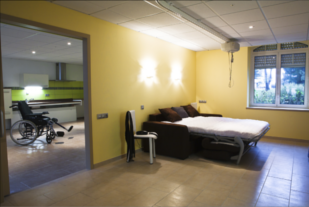
\includegraphics[scale=1]{1-PreEtude/img/appt_tremplin_intro.png}
	\caption{Appartement tremplin : chambre}
	\label{appart}
\end{figure}

Lors de ce rapport, nous allons étudier les spécifications de notre projet, nous allons pour cela les séparer en deux catégories. Tout d'abord, les spécifications fonctionnelles du projet, c'est-à-dire le contenu du logiciel tels que la gestion de périphériques spécifiques ou les différents scénarios. Ensuite, celles au niveau de l'utilisateur, il s'agit des contraintes quant à l'ergonomie pour les patients ainsi que pour le thérapeute. Nous allons enfin faire une ébauche de l'architecture générale du logiciel, où nous ferons une liste des différentes briques logicielles que nous utiliserons et détaillerons comment les elles sont reliées.


